\section{Gestion d'erreurs}

	Dans la programmation système, on manipule tout ce qui touche au système d'exploitation. Ainsi, on doit souvent faire face à des codes d'erreurs. La gestion des erreurs est donc un élément primordial dans la programmation système.
	
	\subsection{Le flux d'erreurs standard}
		Le flux d'erreurs standard \lstinline!stderr! se modélise par un fichier dans lequel on peut écrire nos erreurs. Grâce à cette écriture séparée, l'utilisateur pourra rediriger le flux standard afin d'isoler les erreurs et ainsi mieux les traiter, en nombre moins importants, devant la masse d'informations contenues en sortie. 
		
		\subsubsection*{Les flux standards :}
			Il existe 3 flux standards qui régissent l'utilisation d'un processus d'un programme écrit en C.
			
			\paragraph{} Les flux peuvent être représentés comme des canaux dans lesquels circulent des informations. Dans l'informatique moderne, ces flux sont représentés par l'abstraction de base du disque dur : le fichier. Ainsi, tout ce qui sera écrit dans un des flux sera écrit dans le fichier associé. À l'origine modélisés sur des systèmes d'exploitation de type UNIX , cette technique s'est largement généralisée auprès des systèmes d'exploitation modernes. D'une manière plus générale, on peut associer la notion de flux à d'autres flux plus renommés : flux RSS, flux de paquets, etc.
			
			\paragraph{} En programmation, l'utilité principale des flux réside dans les entrées/sorties. On distingue trois flux standards : 
			\begin{itemize}
				\item le flux d'entrée standard \lstinline!stdin!
				\item le flux de sortie standard \lstinline!stdout!
				\item le flux de sortie d'erreurs standard \lstinline!stderr!
			\end{itemize}
			Le fichier d'en-tête \lstinline!<stdio.h>! déclare ces identificateurs comme étant de type pointeurs sur \lstinline!FILE!.
			
			\begin{center}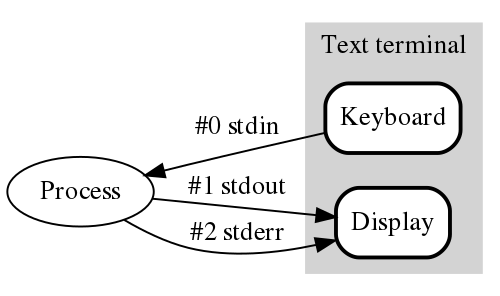
\includegraphics[scale=0.4]{../img/stdStreams.png}\end{center}
			
			Ces 3 descripteurs de fichiers sont initialisés au lancement du processus, et sont libérés à sa destruction. Il n'est donc pas nécessaire de les ouvrir et de les fermer comme on pourrait le faire avec des fichiers classiques.\\
			Le flux d'entrée standard est tout ce qui est envoyé en entrée au programme sous la forme d'informations écrites au clavier en général. Toutefois, l'entrée standard peut prendre une forme différente dans le cadre d'une redirection.\\
			Le flux de sortie standard et le flux de sortie d'erreurs standard sont par défaut associés à la console. Il est possible de les isoler l'un de l'autre, afin de différencier messages d'informations, envoyés à la sortie standard, et messages d'erreurs ou avertissements, envoyés à la sortie d'erreurs standards.
			
			\paragraph{Redirection d'un flux :} l'utilité concrète des trois flux est attribuée à l'utilisateur. En effet, celui-ci peut rediriger un ou plusieurs des trois flux vers un fichier. 
			\begin{itemize}
				\item La redirection du flux d'entrée standard peut permettre de soumettre à un programme une batterie de tests sans avoir à retaper les mêmes entrées. 
				\item La redirection du flux de sortie standard peut permettre d'enlever tous les messages inutiles que certaines applications affichent.
				\item La redirection de flux de sortie d'erreurs standard peut permettre à l'utilisateur d'isoler les erreurs, et ainsi de les traiter pertinemment.
			\end{itemize}	
			Parmi les techniques de redirection :
			\begin{itemize}
				\item \lstinline!1>! redirige la sortie standard vers un fichier passé en paramètre à la suite du symbole 
				\item \lstinline!2>! redirige la sortie d'erreurs standards vers le fichier
				\item \lstinline!<! redirige l'entrée standard vers un fichier
			\end{itemize}
			
			\begin{lstlisting}
				#include <stdio.h>
				
				int main(void) {
					printf("hello world\n");
					return 0;
				}
			\end{lstlisting}
			
			\begin{lstlisting}[style=terminal]
				$ gcc hello.c -o hello.out
				$ ./hello.out 1> hello.txt
				$ cat hello.txt
				hello world !
			\end{lstlisting}
			
			
	\subsection{La variable globale \ttfamily{errno}}
	
		Pour signaler une erreur, les fonctions renvoient une valeur spéciale, indiquée dans leur documentation. Celle-ci est généralement \textbf{-1} (sauf pour quelques exceptions). La valeur d'erreur alerte l'appelant de la survenance d'une erreur, mais elle ne fournit pas la description de ce qui s'est produit. La variable globale \lstinline!errno! est alors utilisée pour en trouver la cause. Cette variable \lstinline!errno! est donc le point de départ de la gestion des erreurs standard offerte par la bibliothèque standard de C. 
		
		\begin{lstlisting}
			#include <errno.h>

			extern int errno;
		\end{lstlisting}
		
		Sa valeur est valable uniquement juste après l'utilisation de la fonction que l'on veut tester. En effet, si on utilise une autre fonction entre le retour que l'on veut tester et l'exploitation de la variable de \lstinline!errno!, la valeur de \lstinline!errno! peut être modifiée entre temps. Elle contient donc une valeur correspondant au code de la dernière erreur s'étant produite.
		
		\subsubsection*{Interprétation du contenu de \lstinline!errno! :}
			À chaque valeur d'erreur possible de \lstinline!errno! correspond une constante du préprocesseur, dont la description est disponible dans le manuel (\lstinline!man errno!).
			
			\paragraph{} La bibliothèque standard ne définit que trois codes d'erreur : \textbf{\textit{EDOM}} (passage en paramètre en dehors du domaine attendu), \textbf{\textit{ERANGE}} (résultat trop grand ou trop petit) et \textbf{\textit{EILSEQ}} (erreur de transcodage). Cependant, les systèmes d'exploitation communs et actuels proposent souvent certaines extensions au contenu de \lstinline!errno!. La norme \textbf{\textit{POSIX}} définit par exemple une trentaine de constantes numériques supplémentaires.
			
			\paragraph{} Il est donc difficile d'associer directement le contenu de \lstinline!errno! à des codes d'erreur, car la portabilité risque de nous faire défaut. C'est pourquoi la bibliothèque standard de C met à disposition deux fonctions qui interprètent le contenu de \lstinline!errno!, évitant ainsi de passer par un code non standard, ou bien considérablement allongé.
			
			\paragraph{La fonction \lstinline!strerror! :} associe au code d'erreur passé en paramètre une description de celui-ci.
				\begin{lstlisting}
					#include <string.h>
					
					extern char* strerror(int errnum);
				\end{lstlisting}
			
			\paragraph{La fonction \lstinline!perror! :} plus utilisée et plus simple d'usage, associe à la valeur courante de \lstinline!errno! sa description, l'affichant sur la sortie d'erreurs standard \lstinline!stderr!. Il est également possible de placer un préfixe \lstinline!s! devant cette description, que l'on pourra passer en paramètre.
				\begin{lstlisting}
					#include <stdio.h>
					
					extern void perror(const char* s);
				\end{lstlisting}
				
				\begin{lstlisting}
					if (fork() == -1) {
						perror("fork");
					}
					//Affiche "fork : Description de l'erreur"
				\end{lstlisting}

			
			
			
		
			
			
			
			
			
			
			